\section{Layout and execution of the experiment}
As mentioned above we will analyse the different characteristic of our CCD, do some of the basic data reduction and determine the bandgap of silicone. Afterwards we will create a CMD from archive pictures of a globular cluster and fit an \textit{isochrones} to determine its age metallicity as well as the distance modulus. The suggested schedule from \cite{manual} intends for us to make an observation ourself, process and analyse it. But since the weather was not fitting in the 3 days we booked the experiment, we didn't get to make said observation.
\vspace{3mm}\\
\subsection{CCD and telescope}
We use the \textbf{KING} (\textbf{K}önigsstuhl \textbf{I}nstrument of \textbf{n}ight-sky \textbf{g}azing) telescope located at the MPIA, Heidelberg, shown in figure \ref{tele}. Its main mirror is 70 cm diameter and focuses parallel light into the CCD detector, which is a \textit{Loral/Lesser n2k2eb BI} thinned and back illuminated CCD. It has 2048 x 2048 pixel with a size of 3 cm x 3 cm resulting 15 $\mu$m per pixel and a quantum efficiency of up to 90\%. We will operate it with 4 pixel counting as 1 since we aren't interested in the high resolution in this experiment. The filters, the shutter and the CDD detectors itself will be controlled from a UNIX computer via terminal. The flat surface needed will be provided by a white sheet hanging on the wall of the dome as shown in figure \ref{flat_white}. \\
\begin{figure}[h]
	\begin{subfigure}{0.5\textwidth}
	\centering
	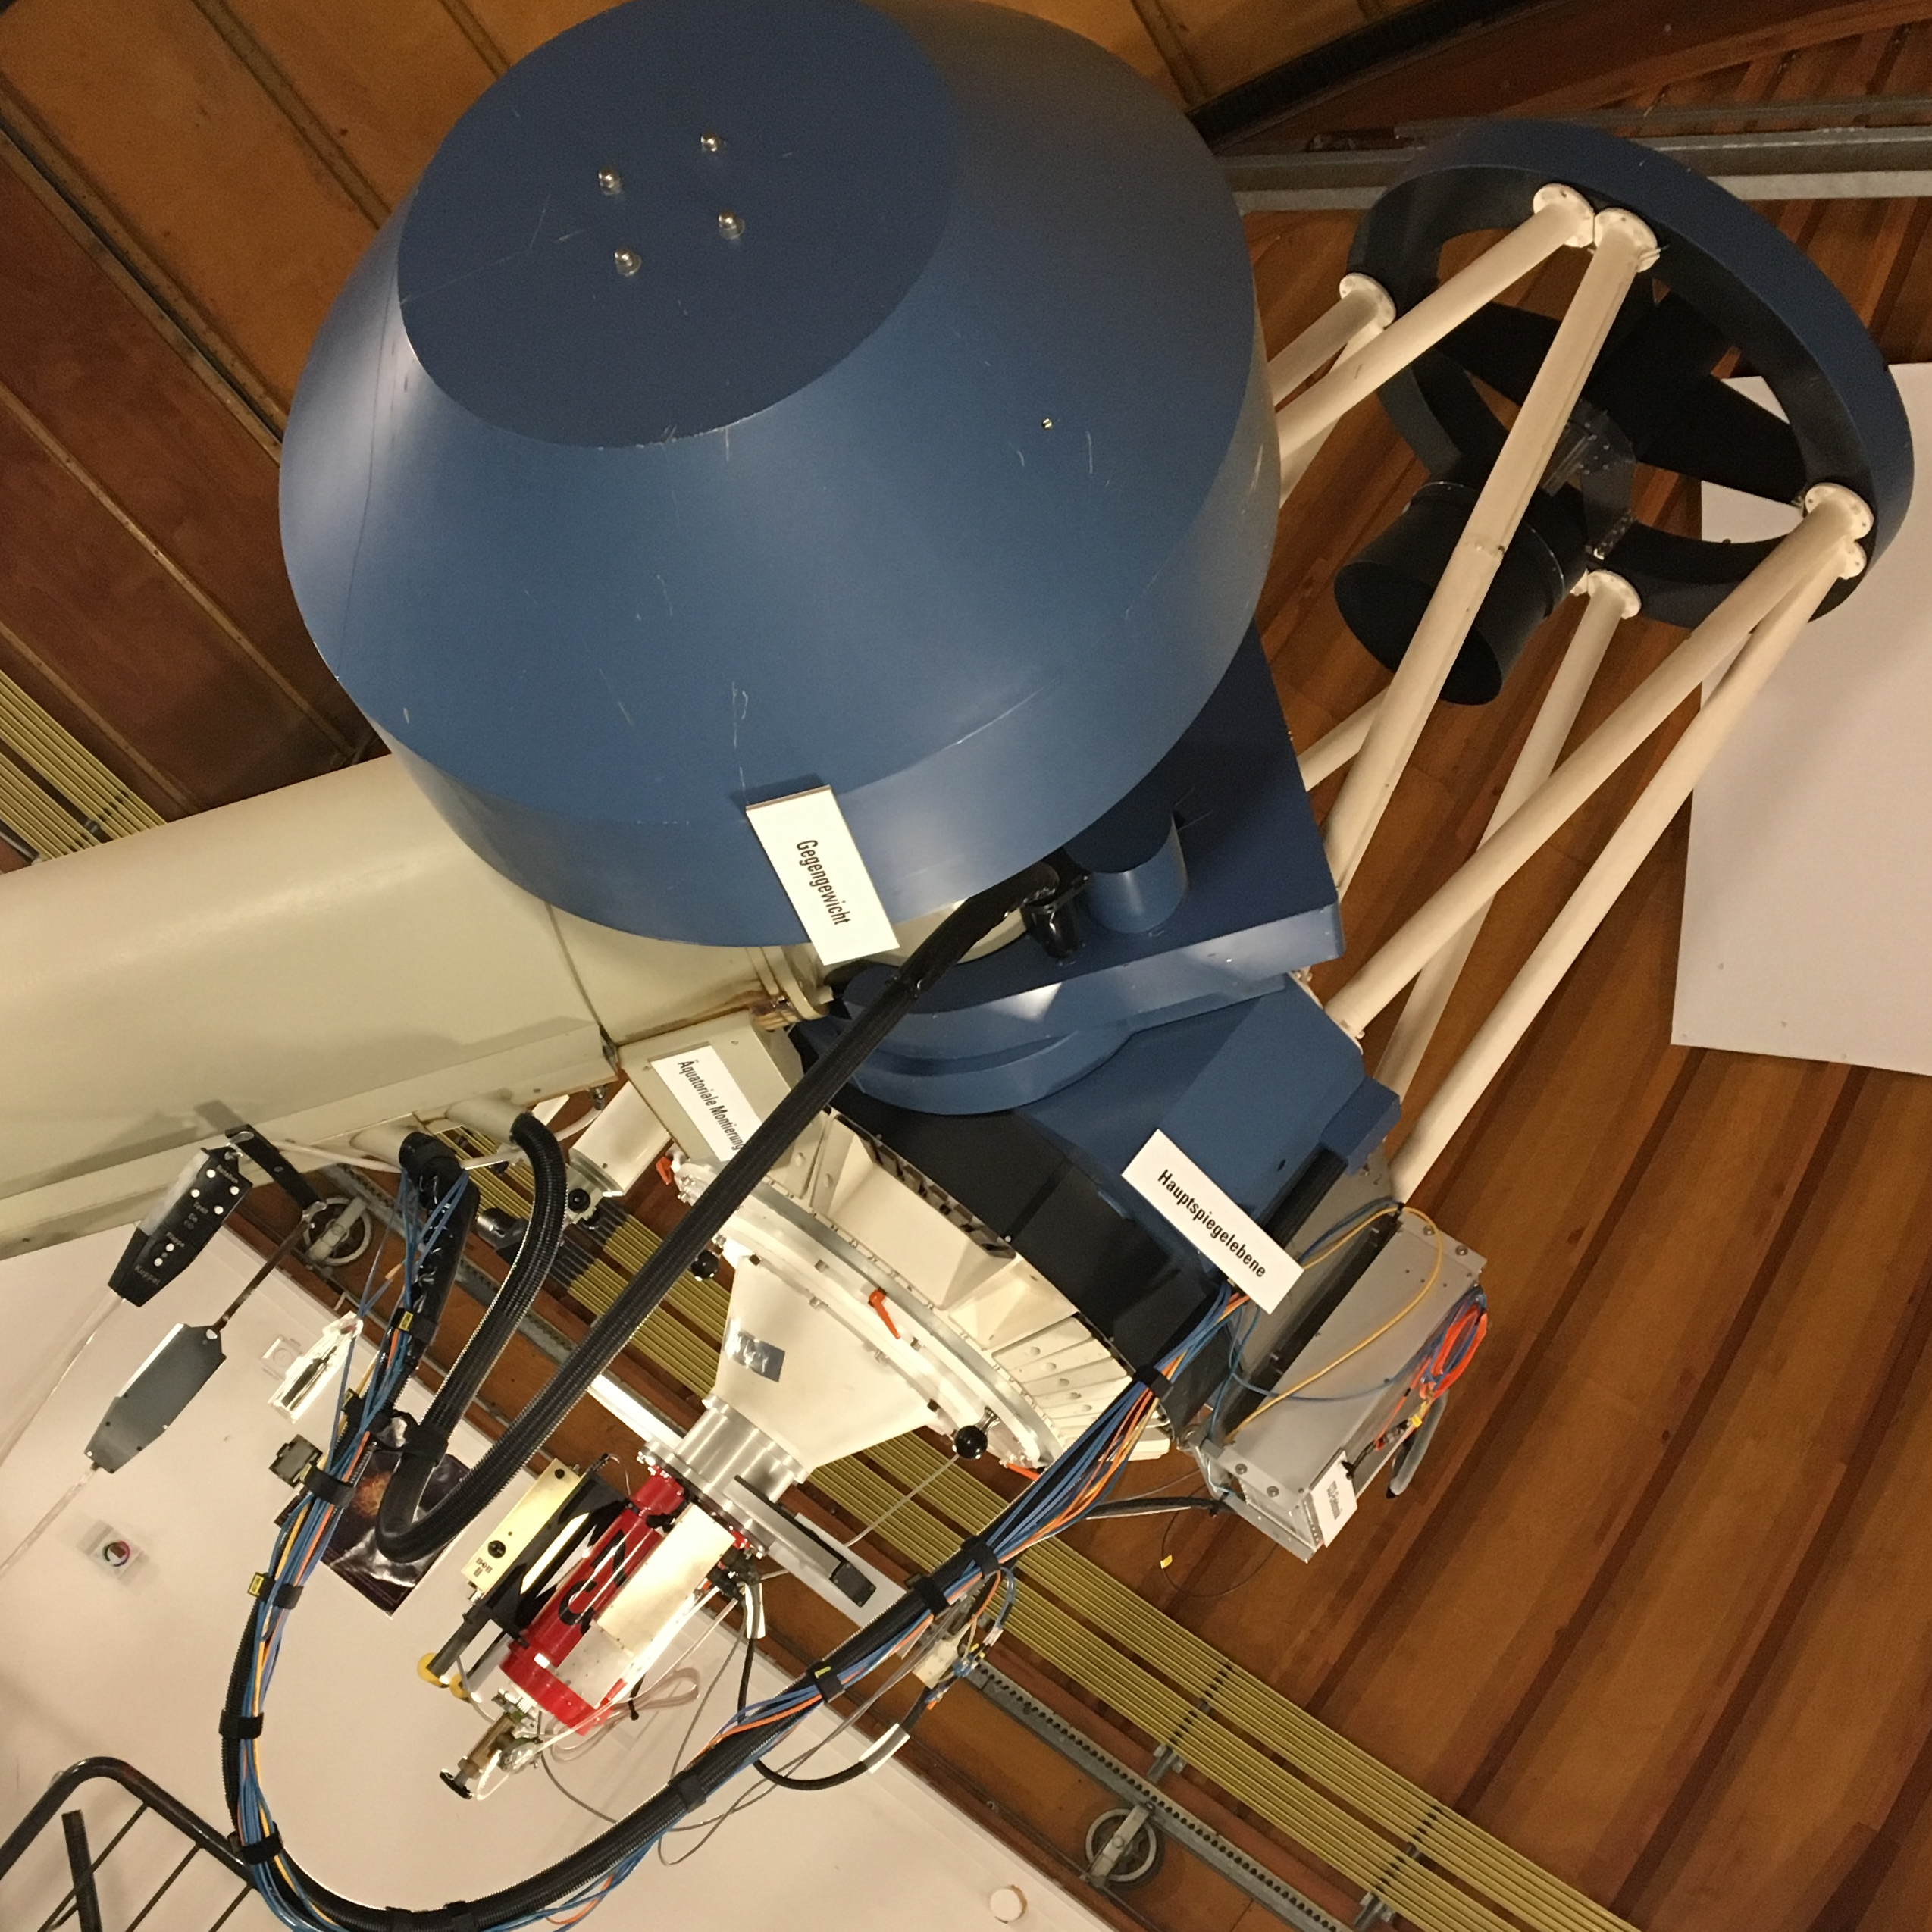
\includegraphics[width=0.8\linewidth]{report_pictures/IMG_1346.png}
	\caption{KING with CCD in the red box}
	\label{tele}
	\end{subfigure}
	\begin{subfigure}{0.5\textwidth}
	\centering
	\includegraphics[width=0.8\linewidth]{report_pictures/IMG_1351.png}
	\caption{Flat surface for flat-field}
	\label{flat_white}
	\end{subfigure}
	\caption{Pictures taken from KING and the dome where it is located}
\end{figure}
\vspace{3mm}\\
\subsection{Execution of the measurements}
Firstly we need to cool the CCD detector. For that purpose, we evacuate the vessel containing the chip to around $10^{-6}$ mBar and fill it with liquid nitrogen. Before starting the cooling process we make ourselves familiar with the process of taking an image and write a macro to take images for us with constant exposure time in equidistant points in time, to observe the cooling process and the dark current. For that measurement it doesn't matter which filter is in use, since we have the shutter closed. Upon reaching our working temperature we make measurements of the flat surface for all 3 filters, as well taking images with increase exposure time in the R filter to check the linearity as well as the saturation area of our the CCD. Afterwards we take pair images with increasing exposure time in the I filter for noise analysis as discussed in section \ref{noise}. 
\vspace{3mm}\\
\subsection{Analysing archive data from BS90}
In the second part we analyse archive pictures from the globular cluster BS90. They were taken July 13th - 18th 2004 from the Hubble Space Telescope (HST) with the filters F555W (V) and F814W (I) \cite{HST_visit_report}. For that matter we will firstly we determine the counts of bright stars in the image which are also in the star catalogue in \textit{SIMBAD}. Then with apparent magnitude from the catalogue and the counts from our pictures we can determine the zeropoints for each picture, i.e. filter.
\vspace{3mm}\\
Since detecting all stars manually takes way too long, we use the program \textit{STARFINDER}. We first analyse the Noise of the each picture, since the program takes the noise into account for the threshold what it registers as a star. Afterwards we create a PSF by showing the program roughly 10 \textit{example stars}. After limiting the size of the PSF to 50 pixel and normalizing it we start the iterative process of star finding where it scans the whole picture to find objects similar to that of the PSF, where we set a lower bound threshold relative to the noise. After doing that for both pictures individually we use a python script to match found stars from both lists by using a max deviation of 1 pixel. This matched star list now contains stars where apparent magnitude of both filters are known. Afterwards we can plot a CMD from that and fit an \textit{isochrone} to it to determine age, metalicity and distance of BS90.
\vspace{3mm}